\documentclass[aps,12pt,prd,nofootinbib,bibnotes, amsmath,amssymb,showpacs,superscriptaddress,floatfix]{revtex4-2}
\bibliographystyle{apsrev}
\usepackage[utf8]{inputenc}
\usepackage{epsf,epsfig,graphics}
\usepackage{graphicx,amsmath,mathrsfs,amssymb, amsthm,nccbbb,cancel,xcolor,wrapfig,siunitx,longtable,tabularx,CJKutf8,subfigure,float,xspace,physics,esvect,braket,enumitem,url,makeidx}
\usepackage{verbatim,color,ulem}
\usepackage{bm}
\usepackage[mathscr]{eucal}
\usepackage{hyperref}
\usepackage[toc,page]{appendix}
\usepackage[hang, flushmargin]{footmisc}
\usepackage{footnotebackref}

%%%%%%%%%%%%%%%%%%%%%%%%%%%%%%%%%%%%%%%%%%%
\begin{document}
\title{Computational Astrophysics HW2}
\author{Yi-Hsiang Kuo, 110022506}
\date{Oct. 13, 2022}
\maketitle
%\tableofcontents
%%%%%%%%%%%%%%%%%%%%%%%%%%%%%%%%%%%%%%%%%%%
\section{Exercise 2}
(1) I have finished my python code as $pi5.py$ and the screen shot of my result entitled  $result\_pi5.jpg$, the git hub link is \href{https://github.com/kuo1235/Computational-Astrophysics-2022/blob/main/astr660/Homework/HW2/pi5.py}{\bf{here}} \\ 
  
(2) In addition to do the $log_{10}|\epsilon|$ v.s. $log_{10}N$, since I want to see the relative error scales as $\frac{1}{\sqrt{N}}$ more explicitly, I plot 2 tables as FIG. 1 (or $result\_pi5\_error.jpg$ in git hub): \\

\begin{figure}
	\centering
	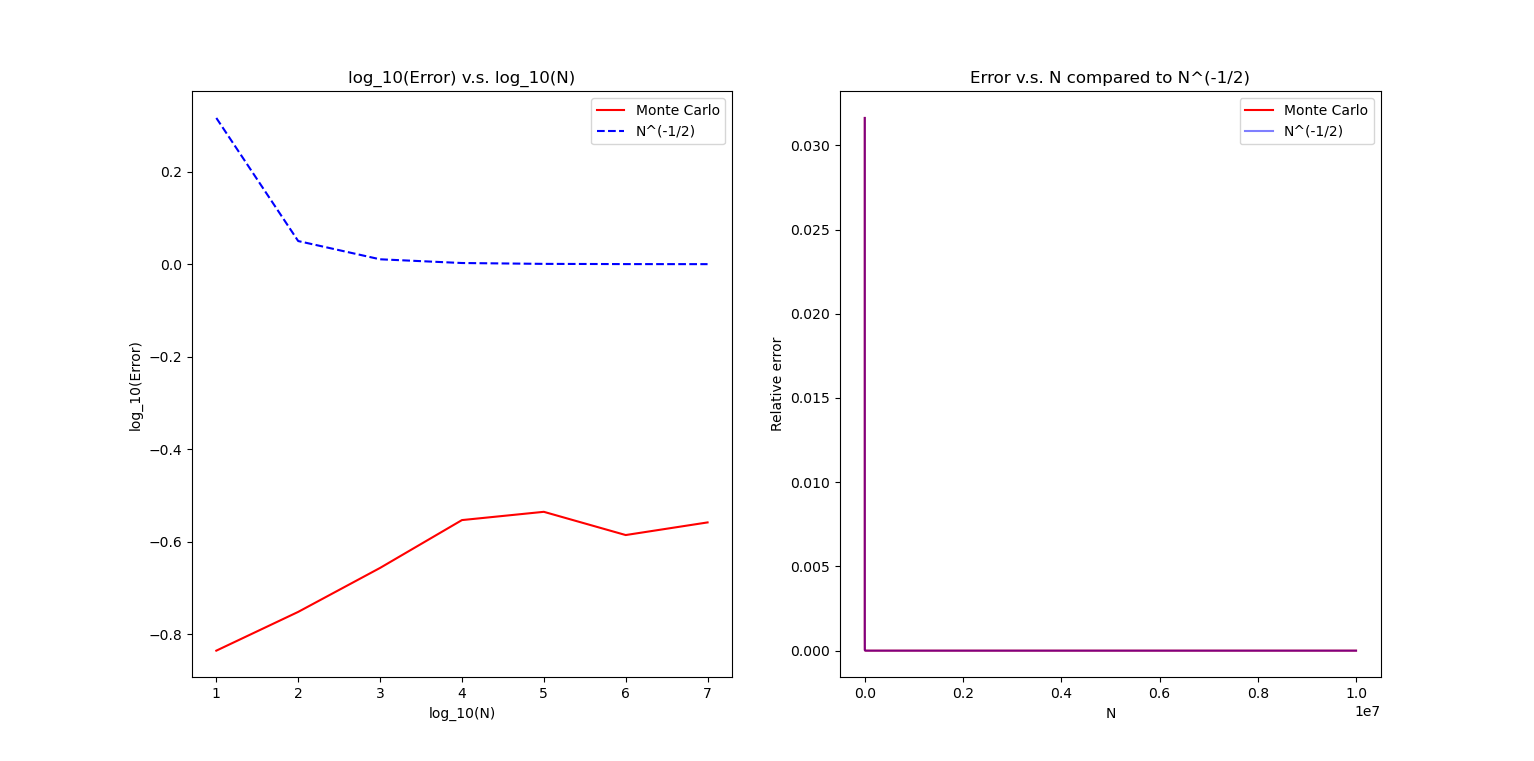
\includegraphics[width=1.0\textwidth]{result_pi5_error}
	\caption{Exercise2-(2) Relative Error figure}
\end{figure}

(3) The modified code adding up a line, we need to do $max\_y \times np.random.rand$ and use this to compute the total area. see FIG. 2 and FIG. 3, and the \href{https://github.com/kuo1235/Computational-Astrophysics-2022/blob/main/astr660/Homework/HW2/Exercise2-(3).py}{\bf{git hub link}}
 
\begin{figure}
	\centering
	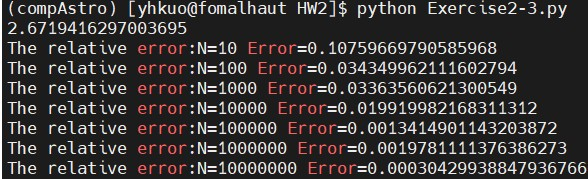
\includegraphics[width=1.0\textwidth]{error_Exercise2-(3)}
	\caption{Exercise2-(3) Relative Error}
\end{figure}

\begin{figure}
	\centering
	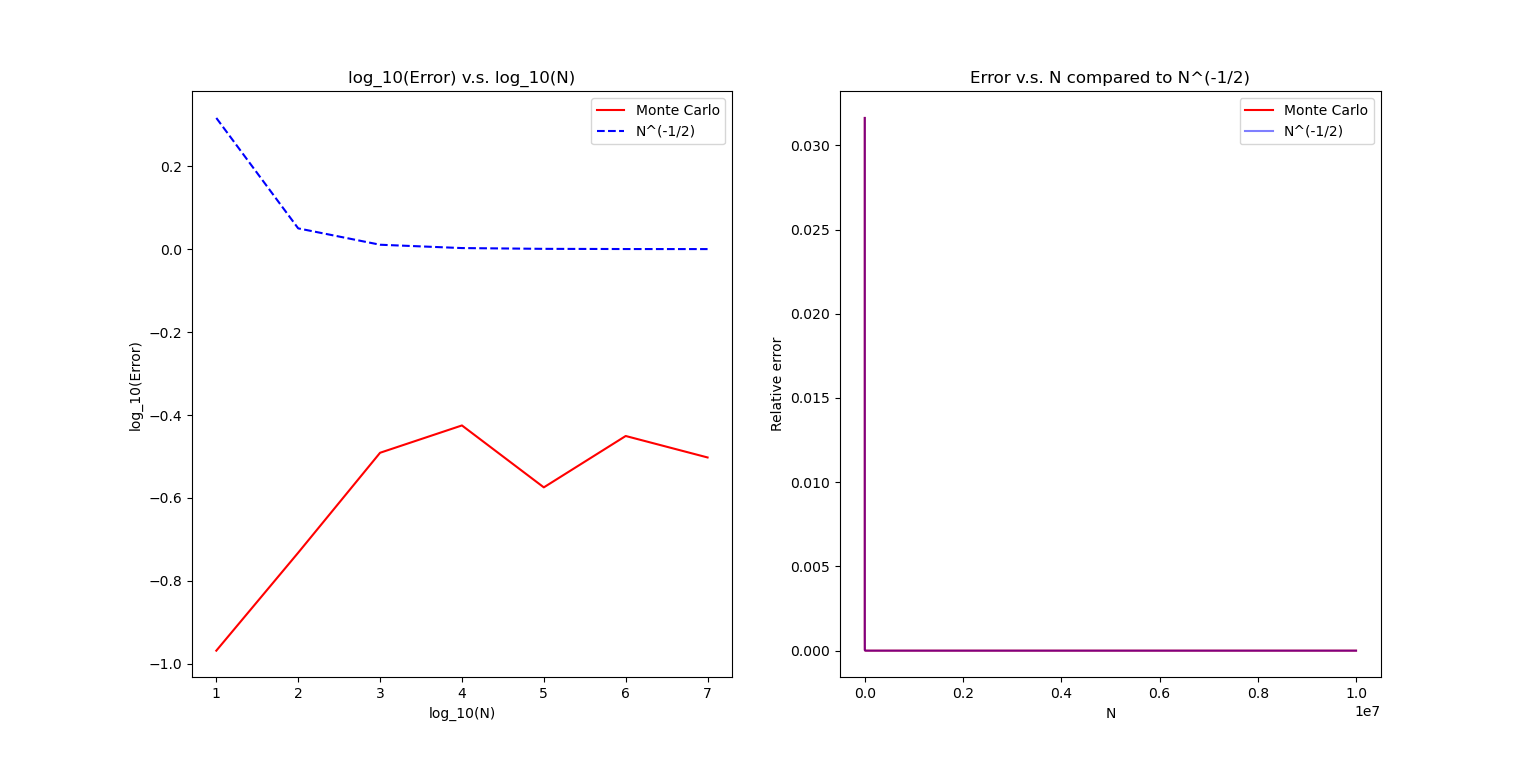
\includegraphics[width=1.0\textwidth]{figure_Exercise2-(3)}
	\caption{Exercise2-(3) Relative Error figure}
\end{figure}

  
\section{Exercise 3}
(1) Find the optimal $N$ where the minimum total error occurs:
\begin{equation}
\epsilon_{tot}=\epsilon_{tr}+\epsilon_{ro} \approx \frac{1}{N^2}+\epsilon_{m} \sqrt{N}
\end{equation}

by doing differentiation, we can find that $N = \epsilon_{m}^{-\frac{2}{5}}$ has extreme value, hence \textcolor{blue}{the optimal $N$ for 32-bit and 64-bit are $1.58 \times 10^{3}$ and $1.0 \times 10^{6}$ respectively}.\\

(2) For Simpson's rule:
\begin{equation}
\epsilon_{tot}=\epsilon_{tr}+\epsilon_{ro} \approx \frac{1}{N^4}+\epsilon_{m} \sqrt{N}
\end{equation}

by doing differentiation, we can find that $N \approx 1.59 \times \epsilon_{m}^{-\frac{2}{9}}$ has extreme value, hence \textcolor{blue}{the optimal $N$ for 32-bit and 64-bit are $5.71 \times 10^{1}$ and $3.43 \times 10^{3}$ respectively}.\\

(3) Putting the optimal $N$ back to the total error, for midpoint and trapezoid method, \textcolor{blue}{the minimal total error for 32-bit and 64-bit are $4.38 \times 10^{-6}$ and $2.00 \times 10^{-12}$ respectively}; for Simpson's rule, \textcolor{blue}{the minimal total error for 32-bit and 64-bit are $8.50 \times 10^{-7}$ and $6.58 \times 10^{-14}$ respectively}. 
    
\section{Exercise 4}

(1) I have completed the $pi4.f90$ and the \href{https://github.com/kuo1235/Computational-Astrophysics-2022/blob/main/astr660/Homework/HW2/Exercise2-(3).py}{\bf{git hub link here}} and the \href{https://github.com/kuo1235/Computational-Astrophysics-2022/blob/main/astr660/Homework/HW2/error.dat}{\bf{output file here}}, with another figure seeing that whether the error scales like $\frac{1}{N^2}$, and FIG. 4. is the result.\\

\begin{figure}
	\centering
	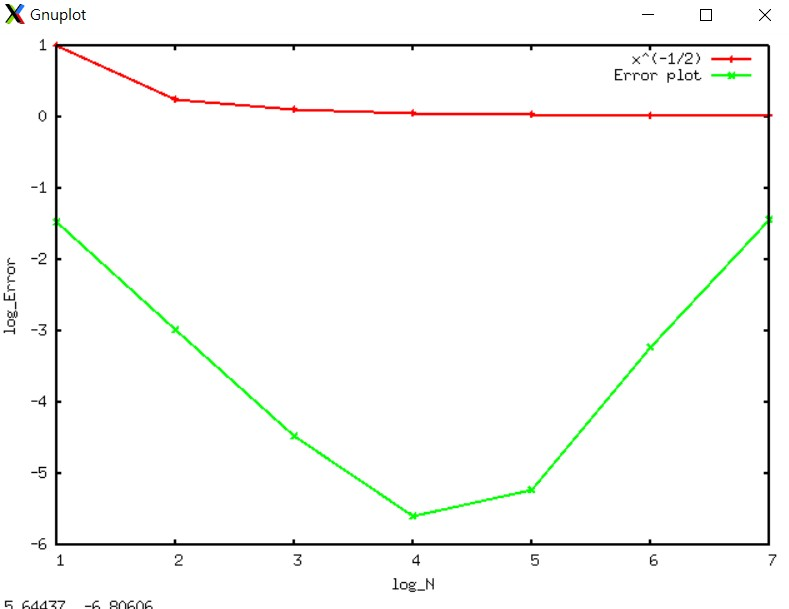
\includegraphics[width=0.8\textwidth]{Exercise4-1}
	\caption{Exercise4-1 Relative Error figure}
\end{figure}

(2)Since we want to see the difference between real(4) and real (8), we need to set our compiler using \textcolor{blue}{\bf{-fdefault-real-8}} while doing the gfortran command. On top of that, according to my answer to Exercise3, the optimal $N \approx 10^6$ and the minimal error $\epsilon_{tot} \approx 2.00 \times 10^{-12}$, this properties can be seen in FIG.5, where $N \approx 10^8$(?) and minimal error indeed $\epsilon_{tot} \approx 10^{-12}$.\\
\begin{figure}
	\centering
	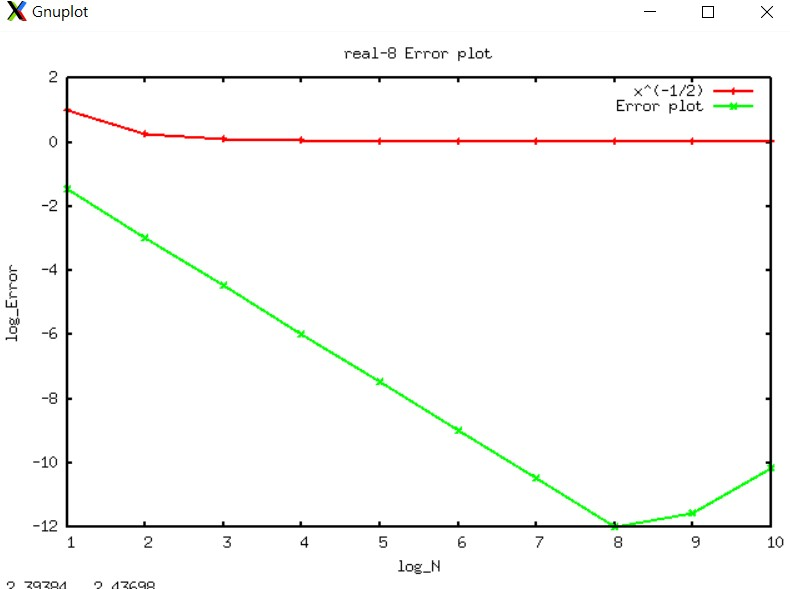
\includegraphics[width=0.8\textwidth]{Exercise4-2}
	\caption{Exercise4-2 real(8) Relative Error figure}
\end{figure}

(3)
for trapezoid method, do the same thing but change the original code a little bit. \href{https://github.com/kuo1235/Computational-Astrophysics-2022/blob/main/astr660/Homework/HW2/trape.f90}{\bf{The code link is here}}, just alter the {\bf{calculate integral part to trapezoid form}}. The results are following figures FIG. 6. and FIG. 7., similar to midpoint method.\\
\begin{figure}
	\centering
	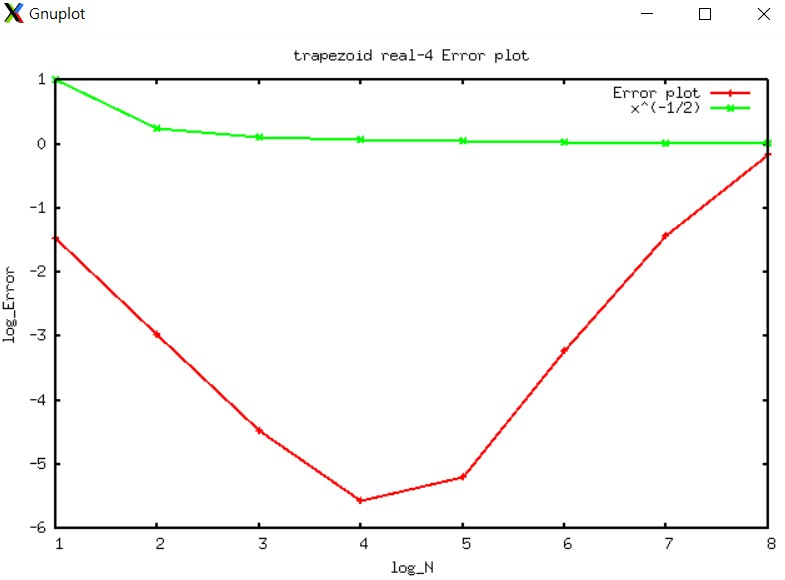
\includegraphics[width=0.8\textwidth]{Exercise4-3_real4}
	\caption{Exercise4-3 real(4) Relative Error figure}
\end{figure}
\begin{figure}
	\centering
	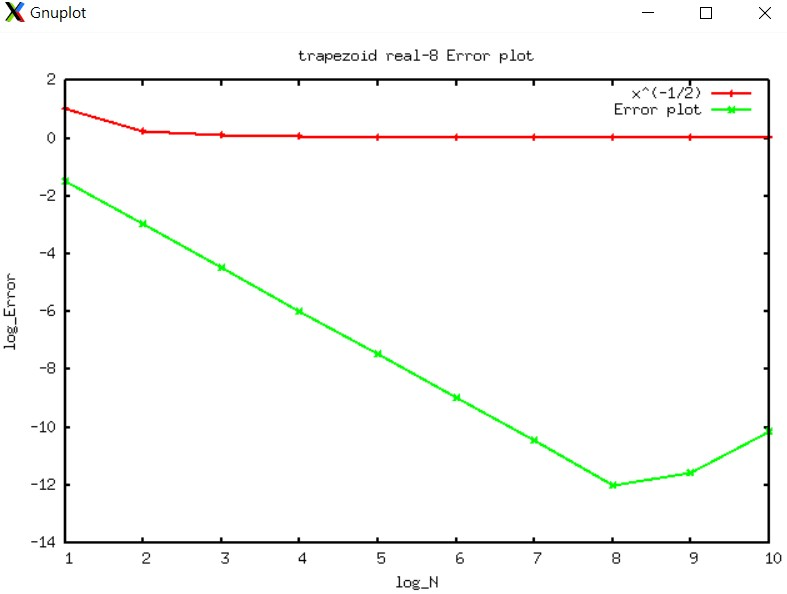
\includegraphics[width=0.8\textwidth]{Exercise4-3_real8}
	\caption{Exercise4-3 real(8) Relative Error figure}
\end{figure}

(4)
for Simpson's method, do the same thing but change the original code a little bit. \href{https://github.com/kuo1235/Computational-Astrophysics-2022/blob/main/astr660/Homework/HW2/simpson.f90}{\bf{The code link is here}}, just alter the {\bf{calculate integral part to Simpson's form}}. The results are following figures FIG. 8. and FIG. 9., according to my answer to Exercise3, {\bf{(32-bit)}}the optimal $N \approx 5.71 \times 10^1$ and the minimal error $\epsilon_{tot} \approx 8.50 \times 10^{-7}$, {\bf{(64-bit)}}the optimal $N \approx 3.43 \times 10^3$ and the minimal error $\epsilon_{tot} \approx 6.58 \times 10^{-14}$. \textcolor{red}{\bf{(result weird?)}}
\begin{figure}
	\centering
	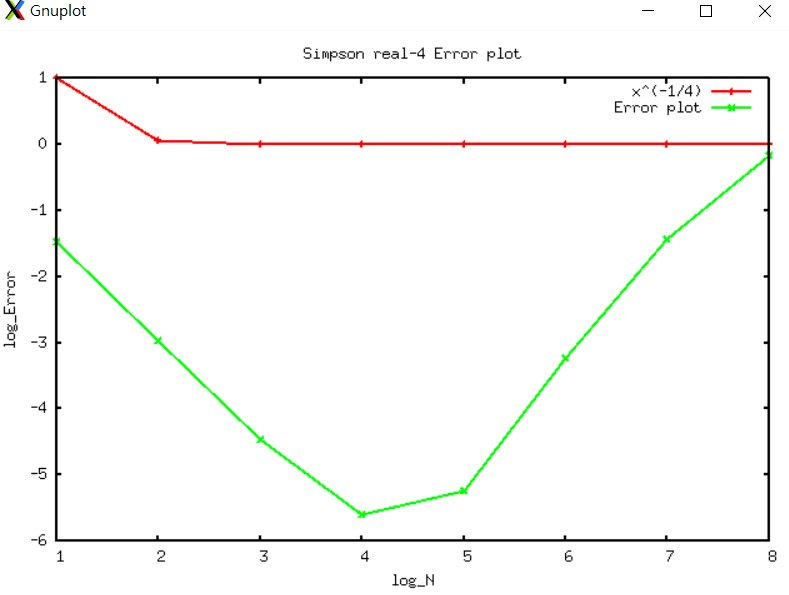
\includegraphics[width=0.8\textwidth]{Exercise4-4_real4}
	\caption{Exercise4-4 real(4) Relative Error figure}
\end{figure}
\begin{figure}
	\centering
	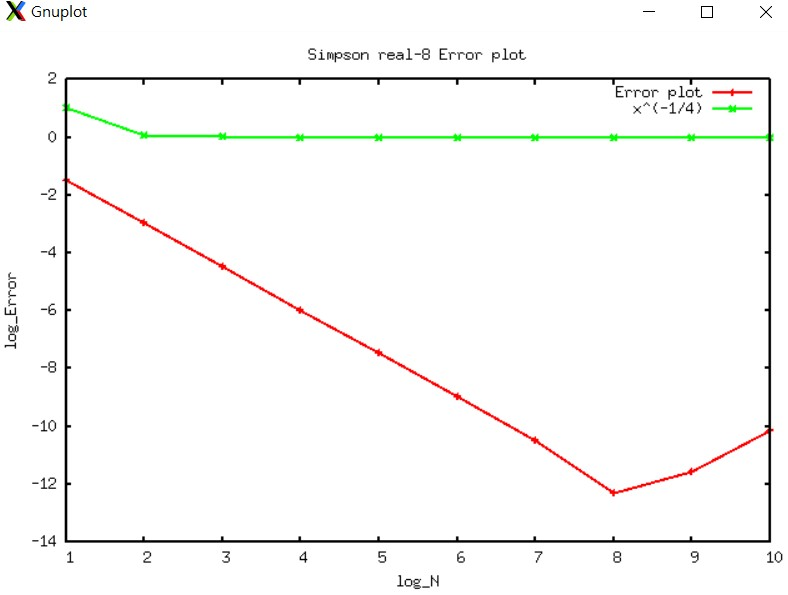
\includegraphics[width=0.8\textwidth]{Exercise4-4_real8}
	\caption{Exercise4-4 real(8) Relative Error figure}
\end{figure}

\section{Exercise 5}
(1)
To find the optimal $h$ which minimize the total error (64-bit):
\begin{equation}
\epsilon_{tot}=\epsilon_{tr}+\epsilon_{ro} \approx \frac{f^{(2)}}{2} h + \frac{\epsilon_{m}}{h}
\end{equation}

Since $f^{(2)} \approx 1$, so after differentiation we find that \textcolor{blue}{\bf{when $h \approx 4.47 \times 10^{-8}$}} \\

(2)
To find the optimal $h$ which minimize the total error of (64-bit) of {\bf{the central-difference algorithm}}:
\begin{equation}
\epsilon_{tot}=\epsilon_{tr}+\epsilon_{ro} \approx \frac{f^{(3)}}{24} h^2 + \frac{\epsilon_{m}}{h}
\end{equation}

Since $f^{(3)} \approx 1$, so after differentiation we find that \textcolor{blue}{\bf{when $h \approx 2.29 \times 10^{-5}$}} \\

(3)Put the optimal h back, we can get the minimal total error for both method, $4.47 \times 10^{-8}$ and $6.55 \times 10^{-11}$ for method 1 and method 2 respectively, {\textcolor{blue}{so method 2 is better behaved}}, also the step size $h$ is smaller for method 2.

\section{Exercise 6}

\bibliographystyle{apsrev}
\bibliography{Ref}
\end{document}








